\documentclass{article}
%\usepackage{geometry}
	%\geometry{margin=1in}
\usepackage{mathtools}
\usepackage{amsthm}
\frenchspacing
\usepackage{multicol}
	\setlength{\columnsep}{-3.5cm}
\usepackage{hyperref}
\usepackage{graphicx}
\usepackage{amssymb}
\usepackage[caption=false]{subfig} %subfigure package 

%\addtolength{\topmargin}{-0.75in}
\setlength{\parindent}{0in}

\usepackage{ifthen}
	\newcommand{\be}{\begin{equation}}
	\newcommand{\ee}{\end{equation}}
	\newcommand{\tab}{\vspace{12pt}}
	\newcommand{\stab}{\vspace{8pt}}
	\newcommand{\bmm}{\begin{bmatrix}}
	\newcommand{\ebm}{\end{bmatrix}}
	\newcommand{\pmm}{\begin{pmatrix}}
	\newcommand{\epm}{\end{pmatrix}}
	\newcommand{\bvm}{\begin{vmatrix}}
	\newcommand{\evm}{\end{vmatrix}}
	\newcommand{\zero}{\mathbb{O}}
	\newcommand{\real}{\mathbb{R}}
	\newcommand{\inte}{\mathbb{Z}}
	\newcommand{\nat}{\mathbb{N}}
	\newcommand{\poly}{\mathcal{P}}
	\newcommand{\all}{\mathbb{C}}
	\newcommand{\ra}{\rightarrow}
	\newcommand{\Dim}{\textrm{dim}}
	\newcommand{\Ker}{\textrm{ker}}
	\newcommand{\spa}{\textrm{span}}
	\newcommand{\Det}{\textrm{det}}
	\newcommand{\al}{\alpha}
	\newcommand{\bt}{\beta}
	\newcommand{\lam}{\lambda}
	\newcommand{\mbf}{}
	\newcommand{\tb}{\hspace{0.5cm}}
	
\renewcommand{\qedsymbol}{$\blacksquare$}

\usepackage[T1]{fontenc}
\usepackage{beramono}
\usepackage{listings}
\usepackage[usenames,dvipsnames]{xcolor}

%%
%% Julia definition (c) 2014 Jubobs
%%
\lstdefinelanguage{Julia}%
  {morekeywords={abstract,break,case,catch,const,continue,do,else,elseif,%
      end,export,false,for,function,immutable,import,importall,if,in,%
      macro,module,otherwise,quote,return,switch,true,try,type,typealias,%
      using,while, global, local},%
   sensitive=true,%
   alsoother={$},%
   morecomment=[l]\#,%
   morecomment=[n]{\#=}{=\#},%
   morestring=[s]{"}{"},%
   morestring=[m]{'}{'},%
}[keywords,comments,strings]%

\definecolor{codegreen}{rgb}{0,0.6,0}
\definecolor{codegray}{rgb}{0.5,0.5,0.5}
\definecolor{codepurple}{rgb}{0.58,0,0.82}
\definecolor{backcolour}{rgb}{0.95,0.95,0.92}

\lstdefinestyle{mystyle}{
    backgroundcolor=\color{backcolour},   
    commentstyle=\color{codegreen},
    keywordstyle=\color{magenta},
    numberstyle=\tiny\color{codegray},
    stringstyle=\color{codepurple},
    basicstyle=\ttfamily\footnotesize,
    breakatwhitespace=false,         
    breaklines=true,                 
    captionpos=b,                    
    keepspaces=true,                 
    numbers=left,                    
    numbersep=5pt,                  
    showspaces=false,                
    showstringspaces=false,
    showtabs=false,                  
    tabsize=2
}

\lstset{style = mystyle}

\title{Exploring the Clifford torus}
\author{Miles Cochran-Branson \\ \small{IHRTLUHC}}
\date{Friday, October 1}

\begin{document}

\maketitle

We will explore the variety $V$ defined by 

\be
	S^1 \times S^1 \subset \real^4. 
\ee

\section*{Implicit Defining Equations}

To begin, we examine the implicit equations that describe this object. Let's first consider the circle $S^1$ which is defined by the set 

\be
	S^1 = \{ (x_1, x_2) : x_1, x_2 \in \real \, | \, x_1^2 + x_2^2 = 1\}. 
\ee

In order to describe our variety, we then take the cartesian product of $S^1$ with itself and find that

\[
	S^1 \times S^1 = \left\{(x_1, x_2, x_3, x_4) : x_1, x_2, x_3, x_4 \in \real \, | \, x_1^2 + x_2^2 = 1 \, \textrm{and} \, x_3^2 + x_4^2 = 1\right\}. 
\]

Thus, we see that our variety is defined by the equations

\be
\begin{split}
	x_1^2 + x_2^2 & = \frac{1}{2} \\
	x_3^2 + x_4^2 & = \frac{1}{2}
\label{eqn:implicit}
\end{split}
\ee

where we have introduced the normalization $x_1^2 + x_2^2 + x_3^2 + x_4^2 = 1$. 

\section*{Parametrization}

Let's now parametrize (3) using trigonometric functions. We first note that 

\be
	S^1 = \{(\cos(\theta), \sin(\theta)) : \theta \in \real \, | \, 0 \le \theta < 2\pi \}. 
\ee

It then follows that

\[
	S^1 \times S^1 = \{(\cos(\theta), \sin(\theta), \cos(\phi), \sin(\phi)) : \theta, \phi \in \real \, | \, 0 \le \theta < 2\pi, 0 \le \phi < 2\pi \}. 
\]

We thus have the parametrized map $f: \real^2 \rightarrow \real^4$ defined by

\be
(\theta, \phi) \mapsto \left(\frac{1}{\sqrt{2}}\cos(\theta), \frac{1}{\sqrt{2}}\sin(\theta), \frac{1}{\sqrt{2}}\cos(\phi), \frac{1}{\sqrt{2}}\sin(\phi)\right)
\label{eqn:param}
\ee

where we have normalized such that the radius of the sphere $\mathbb{S}^3$ is one as above. It is also useful to note here, that this normalization is introduced as our variety $V$ lives within the sphere $\mathbb{S}^3 \subset \real^4$. Thus, we see that we're looking at an object $V \subset \mathbb{S}^3 \subset \real^4$. 

\section*{Computing and Visualization}

\tb Using \verb julia \, we can compute one thousand points that lie on our curve using the following code:

\begin{lstlisting}[language=julia]
using Plots

n = 1000

#Define vectors for input
theta = (2 * pi) .* rand(n)
phi = (2 * pi) .* rand(n)

#Convert to cartesian coordinates
x1 = [(1 / sqrt(2)) * cos(u) for u in theta]
x2 = [(1 / sqrt(2)) * sin(u) for u in theta]
x3 = [(1 / sqrt(2)) * cos(v) for v in phi]
x4 = [(1 / sqrt(2)) * sin(v) for v in phi]
\end{lstlisting}

The output of this can then be turned into a \verb .txt \, file using the \verb DataFrames \, and \verb CSV \, packages in \verb julia . This file, which I have called \verb data_values.txt \,, is included in my project submission. 

\tb We are now tasked with visualizing this object. We will use a stereographic projection so that we can visualize our variety in three dimensions while maintaining as much information as possible. If we project our calculated points from above, which we know lie in $\mathbb{S}^3$, from the three-sphere down into three dimensional space, we can visualize our object. This is done simply through the projection

\be
	(x_1, x_2, x_3, x_4) \mapsto \left( \frac{x_1}{1 - x_4}, \frac{x_2}{1 - x_4}, \frac{x_3}{1 - x_4}\right). 
\ee

Now we can finally plot our object in three dimensions as shown below in Figure 1. 

\begin{figure}[!ht]
	\subfloat[][]{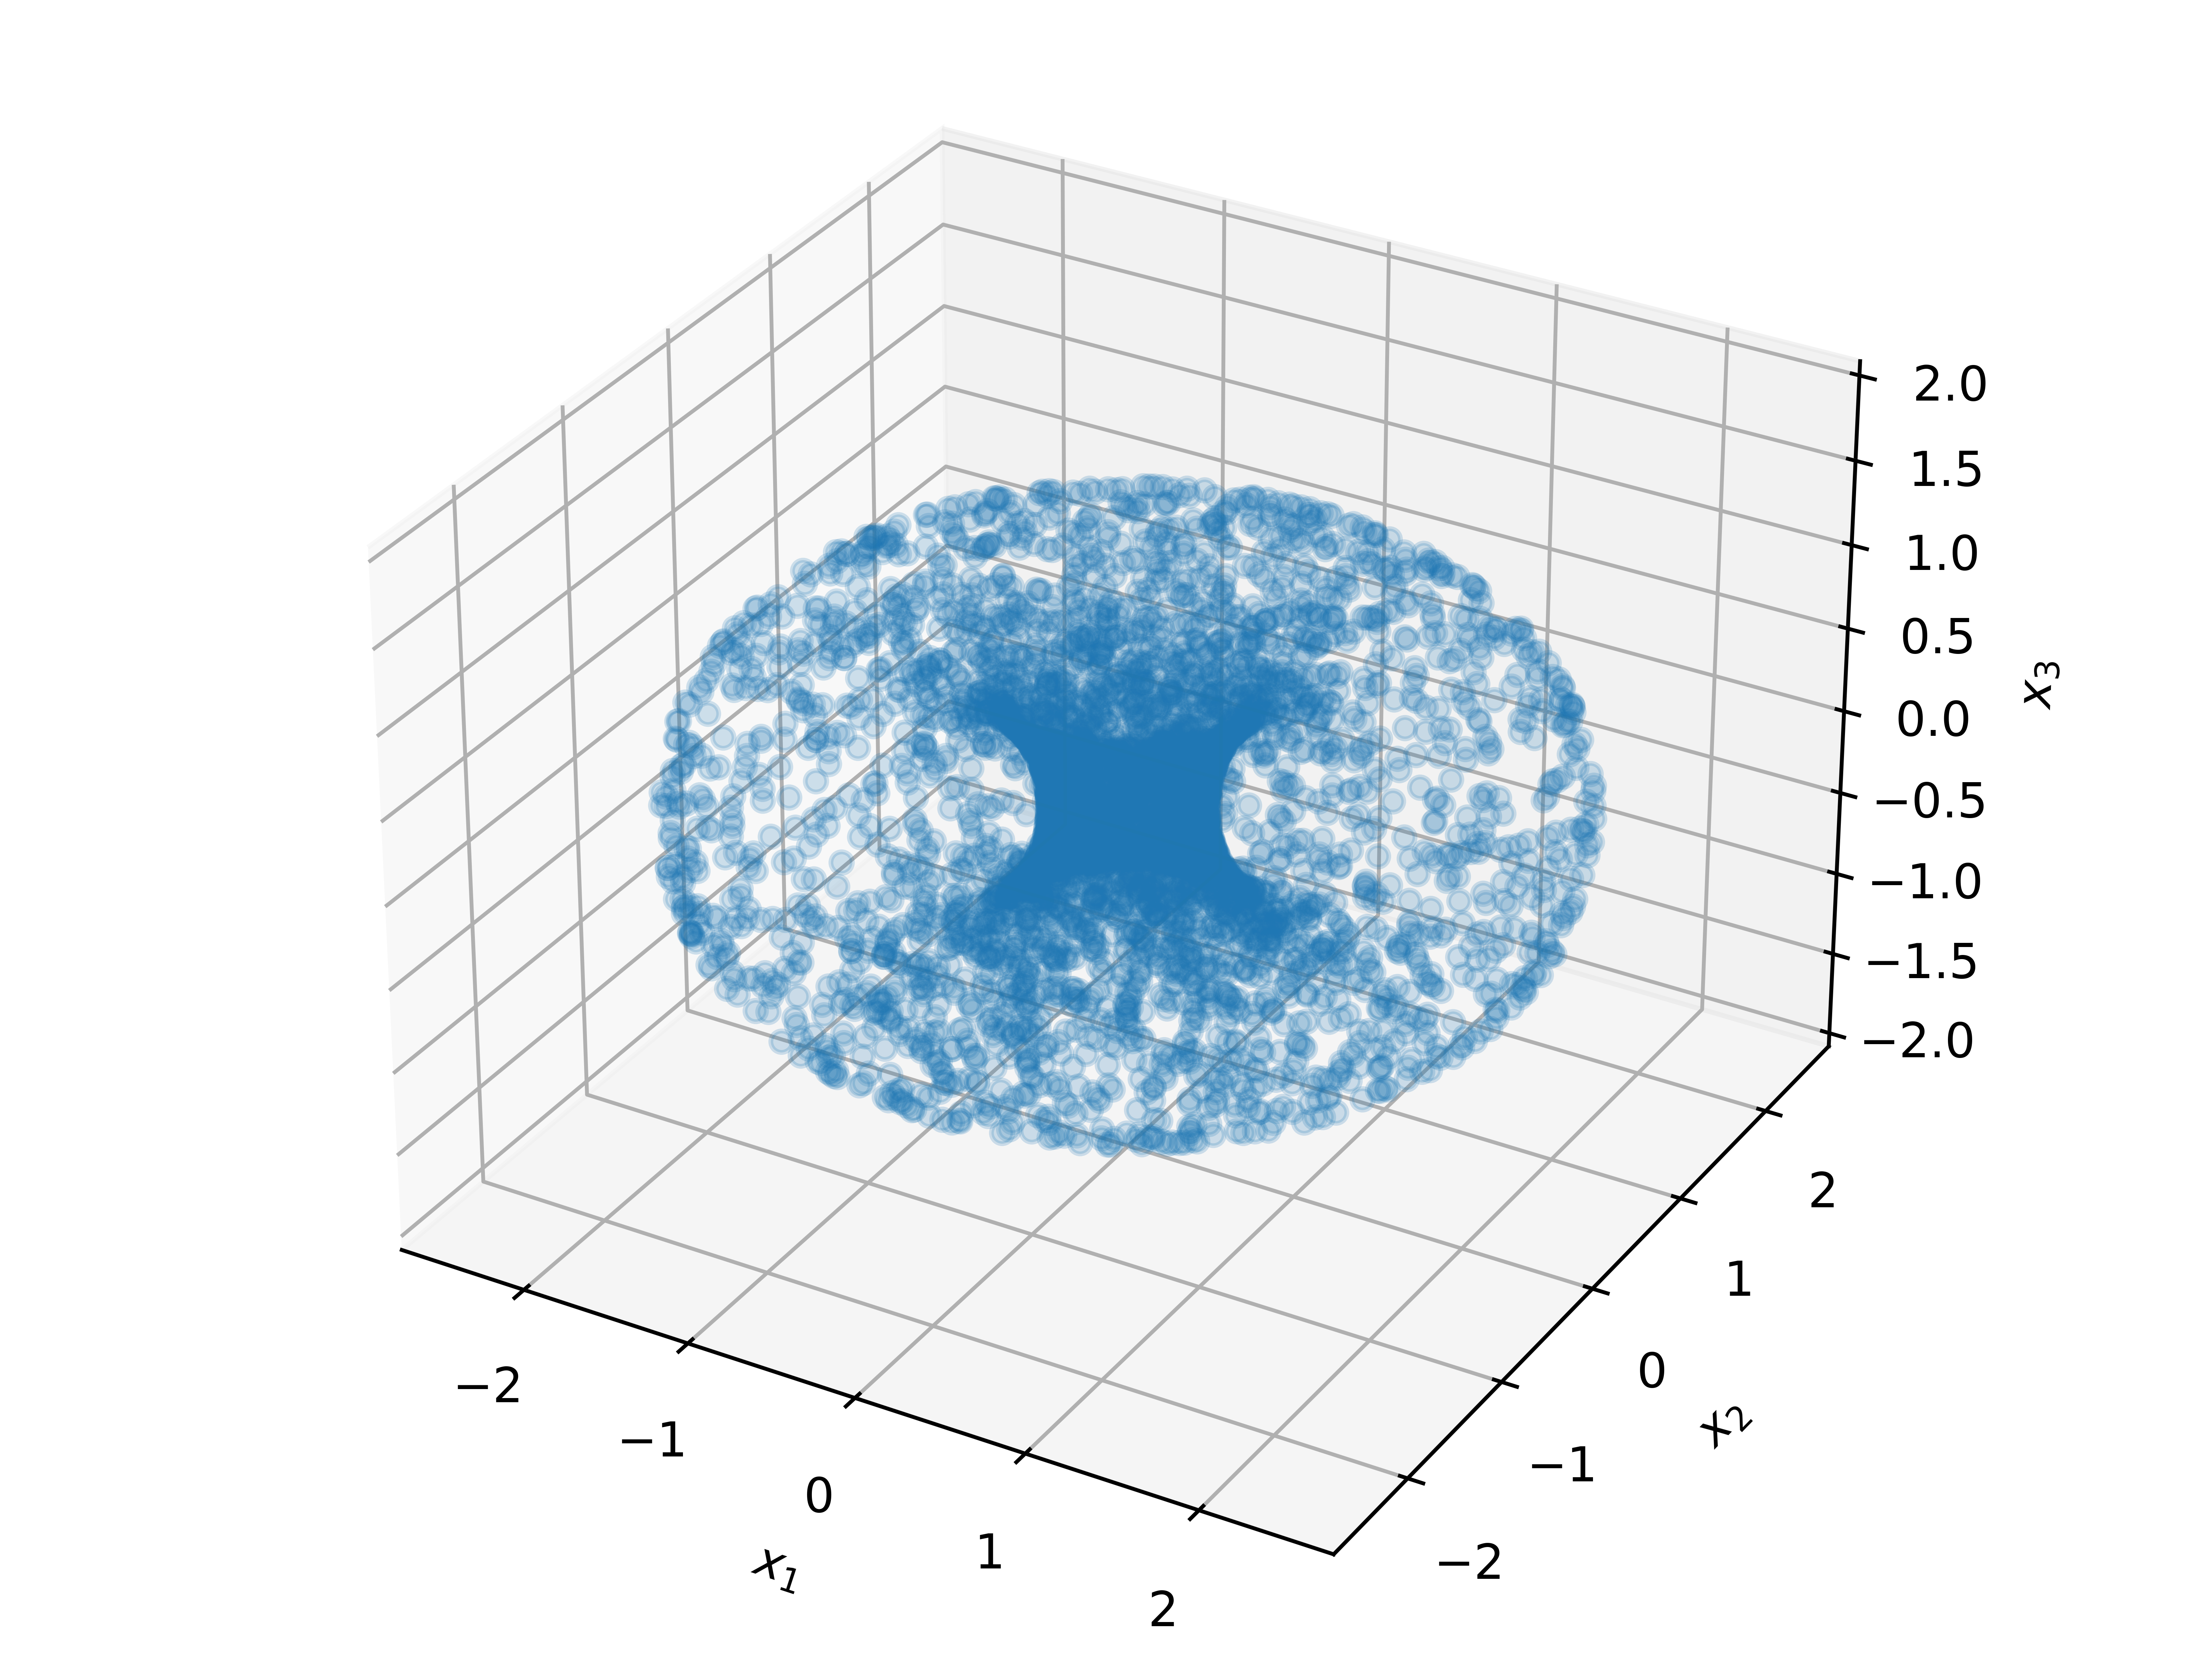
\includegraphics[width = 0.5\linewidth]{torus_plot.png}}
	\subfloat[][]{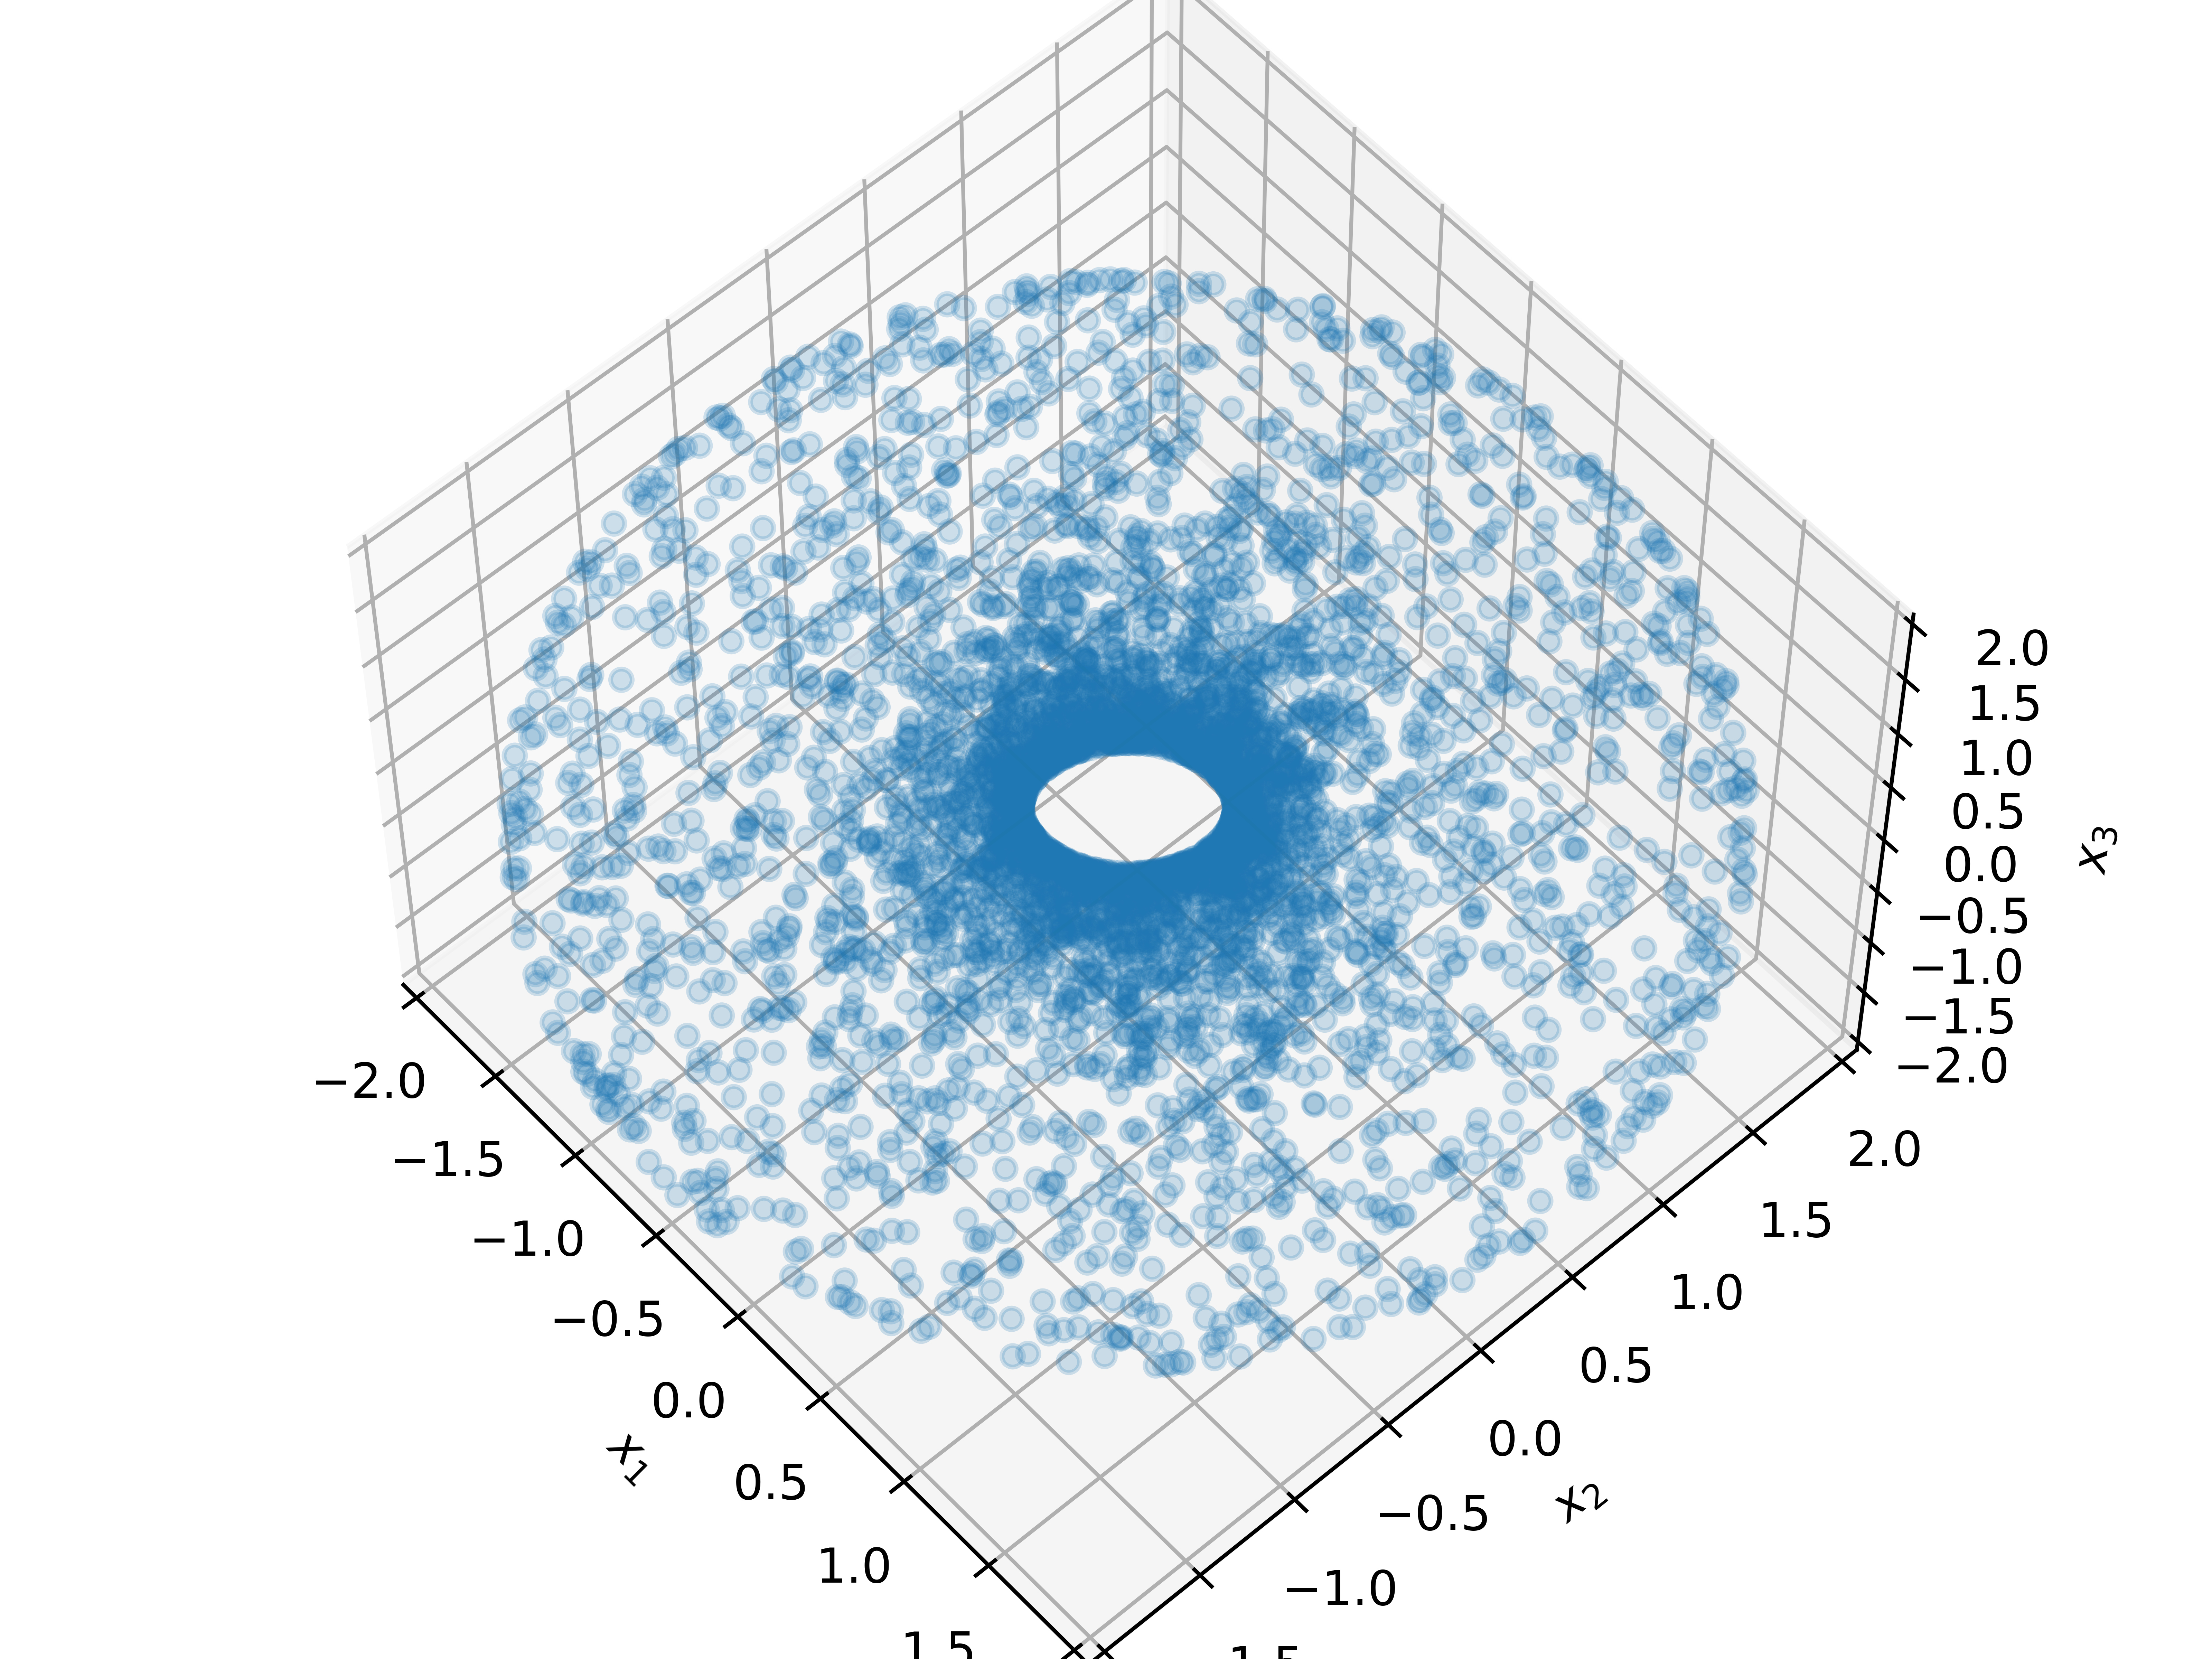
\includegraphics[width = 0.5\linewidth]{torus_plot2.png}}
	\caption{Stereographically projected Clifford torus into three dimensions. (a) shows a side view, while (b) shows a view from the top both of the same object. }
\end{figure}

\tb Of course, this only looks at our object from one point of view. We can rotate the torus in $\real^4$ via the rotation matrix 

\be
	R(\eta) = \pmm \cos(\eta) & -\sin(\eta) & 0 & 0 \\ \sin(\eta) & \cos(\eta) & 0 & 0 \\ 0 & 0 & 1 & 0 \\ 0 & 0 & 0 & 1 \epm. 
\ee

Rotations of our variety executed from $0 \le \eta < 2\pi$ can be projected into $\real^3$ and then visualized through an animation which is included as an attachment to my problem submission. 

\section*{Tangent and Normal Spaces}

\tb Let's now find a basis for both the tangent and the normal space of $V$. In order to find a basis for the tangent space, we compute the derivative of the image of our map, i.e. we compute the derivative of (5) with respect to both $\theta$ and $\phi$. We subsequently find that 

\be
(\theta, \phi) \mapsto \frac{1}{\sqrt{2}} 
					\pmm 
					-\sin(\theta) & 0 \\
					\cos(\theta) & 0 \\
					0 & -\sin(\phi) \\
					0 & \cos(\phi)
					\epm
					\pmm
					v_1 \\
					v_2
					\epm
\ee

where $v_1, v_2 \in \real$ are arbitrary scalers and note that the columns of the above matrix span the tangent space. Thus these columns form a basis of the tangent space. \par

\tb We now consider the normal space and note that a basis for this space can be found by taking the derivate of the image of $V$ given in (3). This is given by 

\be
(x_1, x_2, x_3, x_4) \mapsto \pmm 2x_1 & 2x_2 & 2x_3 & 2x_4 \epm \pmm v_1 \\ v_2 \\ v_3 \\ v_4 \epm
\ee

where, again, $v_1, v_2, v_3, v_4 \in \real$ are arbitrary scalers. We then note that the columns of the above matrix span the normal space which lies in $\real^4$ and thus, the rows of the above matrix form a basis for the normal space. 

\section*{Volume}

In order to compute the volume of our variety, we consider the Gram Matrix which is defined by 

\be
	(G_{\mbf{u}_1, ... , \mbf{u}_k})_{i, j} = \mbf{u}_i \cdot \mbf{u}_j. 
\ee

In this case we're considering $k = 2$, thus

\be
	G_{\mbf{u}, \mbf{v}} = \pmm \mbf{u} \cdot \mbf{u} & \mbf{u} \cdot \mbf{v} \\ \mbf{v} \cdot \mbf{u} & \mbf{v} \cdot \mbf{v} \epm. 
\ee

The vectors $\mbf{v}$ and $\mbf{u}$ are just the basis vectors we found for the tangent space, i.e.

\be
\begin{split}
	\mbf{u} & = \frac{1}{\sqrt{2}}(-\sin(\theta), \cos(\theta), 0, 0) \\
	\mbf{v} & = \frac{1}{\sqrt{2}}(0, 0, -\sin(\phi), \cos(\phi))
\end{split}
\ee

and we see that 

\be
	G_{\mbf{u}, \mbf{v}} = \frac{1}{\sqrt{2}} \pmm 1 & 0 \\ 0 & 1 \epm = \frac{1}{\sqrt{2}} \cdot \mbf{I}. 
\ee

Okay---now from some theorem (which I just found on Wikipedia), we know that 

\be
	Vol_2(V) = \sqrt{\Det(G)}. 
\ee

It's easy to compute the determinant of $G$, namely, 

\be
 \bvm 1/\sqrt{2} & 0 \\ 0 & 1/\sqrt{2} \evm = \frac{1}{2}
\ee

and we see that our volume scale factor from parameter space to $\real^4$ is simply

\be
	Vol_2(V) = \frac{1}{\sqrt{2}}.
\ee

To find the volume of the whole object, we need to integrate over our parameter space. We note that this becomes trivial as $Vol_2(V)$ is constant! Thus, our volume is given by

\be
\begin{split}
	Vol & = \int \!\! \int 1 \cdot \sqrt{\Det G} \cdot dV \\
	& = \int_0^{2\pi} \!\!\!\! \int_0^{2\pi} 1 \cdot \frac{1}{\sqrt{2}} \, d\theta d\phi \\
	& \boxed{ = \frac{4 \pi^2}{\sqrt{2}}}
\end{split}
\ee

\section*{Distance to a point}

Finally, we are tasked with finding the point $p' \in V$ that is closest to the point $(10, 10, 8, 7) \in \real^4$. We can do this computationally by using the distance formula to find the point closest to our object. More specifically, we have to find some $p' = (x_1, x_2, x_3, x_4)$ such that the distance $d$ to the point $p = (10, 10, 8, 7)$ is minimized, where $d$ is given by

\be
d = \sqrt{(x_1 - 10)^2 + (x_2 - 10)^2 + (x_3 - 8)^2 + (x_4 - 7)^2}. 
\ee

This is done by throwing many random points onto our surface to get a range of points from which to sample. We then run through all of these points and find which distance is the smallest. We have thrown $1 \times 10^7$ values for both $\theta$ and $\phi$ and then have found the minimum distance and it's corresponding point using the following function written in \verb julia . 

\begin{lstlisting}[language = julia]
function find_min(n, p)

    #Define vectors for input
    theta = (2 * pi) .* rand(n)
    phi = (2 * pi) .* rand(n)

    #Convert to cartesian coordinates
    x1 = [(1 / sqrt(2)) * cos(u) for u in theta]
    x2 = [(1 / sqrt(2)) * sin(u) for u in theta]
    x3 = [(1 / sqrt(2)) * cos(v) for v in phi]
    x4 = [(1 / sqrt(2)) * sin(v) for v in phi]
	
	  #define distance and minimum point
    d = Inf64
    min_point = Vector{Float64}(undef, 4)    
	
	  #find minimum distance
    for i in 1:n
    d_temp = sqrt((x1[i] - p[1])^2 + (x2[i] - p[2])^2 
    								+ (x3[i] - p[3])^2 + (x4[i] - p[4])^2)
        if (d_temp < d) 
            d = d_temp
            min_point = [x1[i], x2[i], x3[i], x4[i]]
        end;
    end;

    return min_point, d

end;
\end{lstlisting}

Running this function ten times, we get a spread of values for the minimum distance and the point corresponding to this distance. We then append these to a \verb .csv  file, read this into a data frame, and can then compute the standard deviation and our final value for the minimum point. The code for this is shown below

\begin{lstlisting}[language = julia]
#Report average values 
min_distance_avg = sum(df[!, 5]) / length(df[!, 5])
min_distance_std = std(df[!, 5])

#Initialize values for minimizer
d_min = df[1, 5]
min_point = [df[1,1], df[1, 2], df[1, 3], df[1, 4]]

#Find absolute minimum
for i in 2:length(df[!, 1])
    d_temp = df[i, 5]
    if d_temp < d_min
        global d_min = d_temp
        global min_point = [df[i,1], df[i, 2], df[i, 3], df[i, 4]]
    end;
end;
\end{lstlisting}

We find that our minimum distance is given by 

\be
	d = 16.70229639 \pm 0.00000004. 
\ee

and we see that the point closest to $p$ is

\be
\boxed{p' = (0.49998, 0.50001, 0.53215, 0.46594)}
\ee

\end{document}